\section{Retrospettiva}
%Restrospettiva (descrizione finale dettagliata dell'andamento dello sviluppo, del backlog, delle iterazioni; commenti finali)
%Si noti che la retrospettiva è l'unica sezione che può citare aneddoti di cosa è successo in itinere, mentre le altre sezioni fotografino il risultato finale. Se gli studenti decideranno (come auspicato) di utilizzare un product backlog e/o dei backlog delle varie iterazioni/sprint, è opportuno che questi siano file testuali tenuti in versione in una cartella "process", così che sia ri-verificabile a posteriori la storia del progetto.

\subsection{Sprint 1 27/09 - 03/10}
\paragraph{Epic} Visualizzare il personaggio a schermo

Il primo sprint è stato prevalentemente organizzativo ed è stato focalizzato sulla scelta e il setup degli strumenti, la definizione del processo di sviluppo e il design architetturale. 
In particolare si è scelto di lavorare con il framework Indigo e si è studiata la sua documentazione, al fine di comprendere come organizzare il codice e poter definire l’architettura generale del gioco. 
Era previsto anche il setup della CI/CD, abbiamo deciso però di spostarla nella seconda sprint, la quale sarà orientata a implementare la struttura base e produrre la prima schermata di gioco. 


\begin{figure}[!hbt]
    \centering
    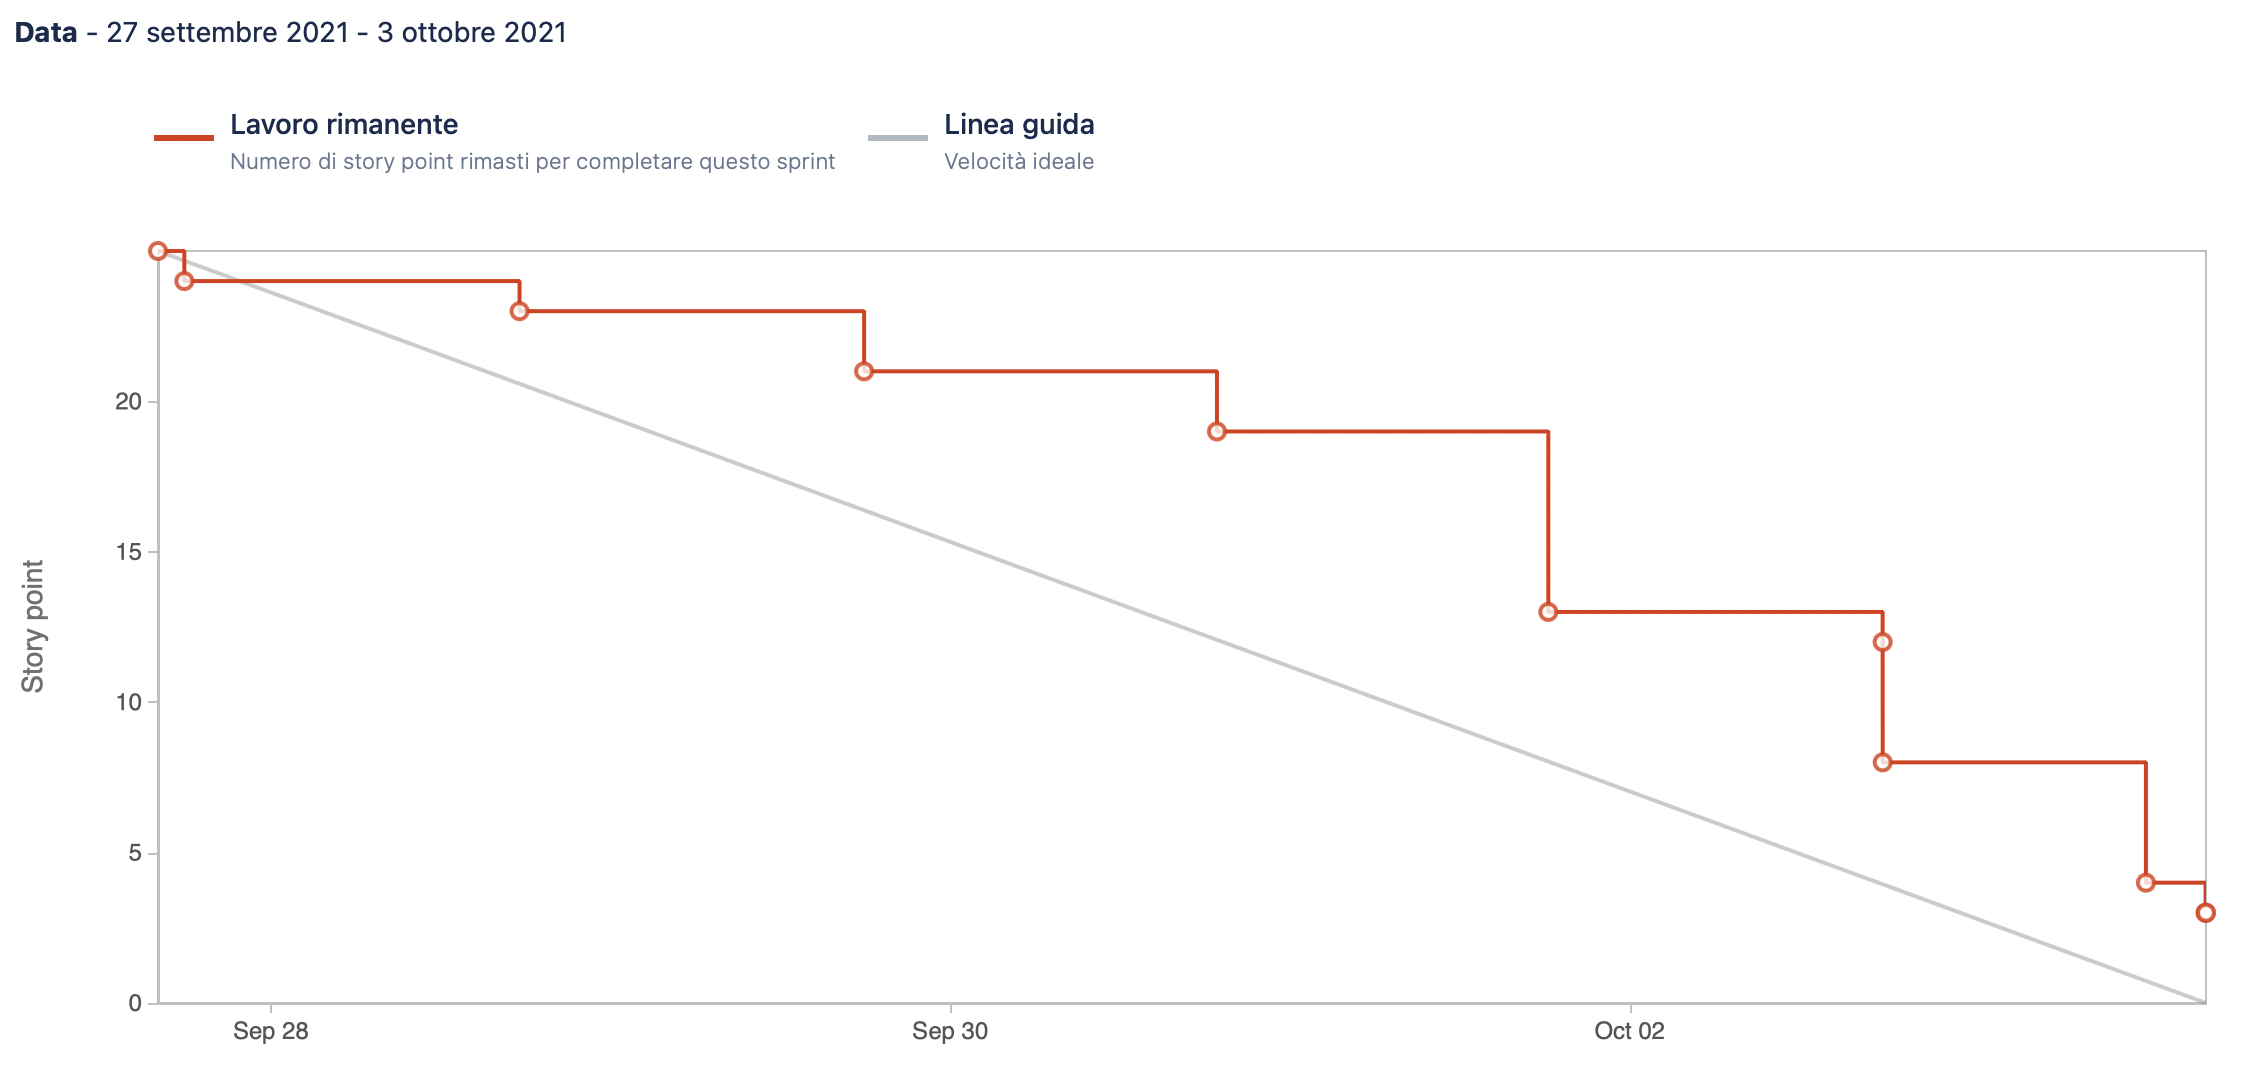
\includegraphics[scale=0.4]{sprint-1-burn-down.png}
    \caption{\textit{Grafico Burn-down primo sprint}} 
\end{figure}


\subsection{Sprint 2}

\subsection{Sprint 3}

\subsection{Sprint 4}

\subsection{Sprint 5}

\subsection{Sprint 6}